\documentclass[11pt]{article}
\newcounter{chapter}
\usepackage{tikz}
\usetikzlibrary{positioning,fit,backgrounds}
\usepackage[normalem]{ulem}
\usepackage{cs1200}

% Solution blocks (always displayed, set in blue so they stand out from the prompt)
\newenvironment{soln}{%
  \par\medskip\noindent\begingroup\color{blue}\textbf{Solution.}\ %
}{%
  \endgroup\par\medskip%
}

% Lyber bipartite graph: drivers 1--6 on the left, customers A--E on the right.
% \lyber{<plain edges>}{<matched edges>}{<augmenting-path edges>}, each a list of d/C pairs.
\newcommand{\lyber}[3]{%
\begin{tikzpicture}[
  every node/.style={circle, draw, minimum size=7mm, font=\small, color=black},
  plain/.style={thin, black},
  matched/.style={very thick, red},
  augpath/.style={line width=5pt, green!70!black, opacity=0.35}
]
  \foreach \d [count=\i] in {1,...,6} \node (d\d) at (0, -1.1*\i) {\d};
  \foreach \c [count=\i] in {A,...,E} \node (c\c) at (5, -1.1*\i - 0.55) {\c};
  \edef\lyberP{#1}\edef\lyberM{#2}\edef\lyberX{#3}%
  % augmenting path is a wide translucent green highlight drawn underneath,
  % so each edge on it still shows as black (unmatched) or red (matched)
  \ifx\lyberX\empty\else\foreach \a/\b in \lyberX {\draw[augpath] (d\a) -- (c\b);}\fi
  \ifx\lyberP\empty\else\foreach \a/\b in \lyberP {\draw[plain] (d\a) -- (c\b);}\fi
  \ifx\lyberM\empty\else\foreach \a/\b in \lyberM {\draw[matched] (d\a) -- (c\b);}\fi
\end{tikzpicture}}
\newcommand{\lyberedges}{1/C, 2/A, 3/A, 3/B, 3/C, 3/D, 3/E, 4/A, 4/D, 5/C, 5/D, 5/E, 6/C}

\begin{document}

% To include a problems set header, use the psHeader command
\psHeader{6}{Thu Nov. 12, 2026 (11:59pm)}

Please see the syllabus for the full collaboration and generative AI policy, as well as information on grading, late days, and revisions.

All sources of ideas, including (but not restricted to) any collaborators, AI tools, people outside of the course, websites, ARC tutors, and textbooks other than Hesterberg--Vadhan must be listed on your submitted homework along with a brief description of how they influenced your work. You need not cite core course resources, which are lectures, the Hesterberg--Vadhan textbook, sections, SREs, problem sets and solutions sets from earlier in the semester. If you use any concepts, terminology, or problem-solving approaches not covered in the course material by that point in the semester, you must describe the source of that idea. If you credit an AI tool for a particular idea, then you should also provide a primary source that corroborates it. Github Copilot and similar tools should be turned off when working on programming assignments.

If you did not have any collaborators or external resources, please write 'none.' A problem set on the border between two letter grades cannot be rounded up if collaborators are not noted.

\vspace{1em}

\textbf{Your name: Andrew Jing}

\textbf{Collaborators and External Resources: Claude added solution sections to LaTeX and turned my drawings into TikZ}

\textbf{No. of late days used on previous psets: 1}

\textbf{No. of late days used after including this pset: 3}

\vspace{1em}

The purpose of this problem set is to practice modeling problems using graphs, reinforce understanding of the matching algorithm we learned, practice the resolution algorithm and reductions to SAT, and think about ethical issues raised when modeling real-world problems for algorithmic solution.

\begin{enumerate}

 \item (Matching Algorithms)
 Another practical application of matching algorithms is planning logistics, like in the following example from (fictional) ridesharing service Lyber in (real) New York City's Times Square.  When a customer books a Lyber ride, the ride request is sent to a Lyber server and combined with others to create a schematic like the one drawn in the map below.

\begin{figure}[h]
    \centering
    \includegraphics[width=0.55\textwidth]{{ps6_diagram.png}}
    \label{fig:travel_time_graph}
\end{figure}

Given a schematic like this, Lyber's goal is to serve as many customers (labeled A--E in the map) as possible, by assigning each one to a driver (labeled 1--6 in the map). For simplicity, each customer and driver is at an intersection, and assume driving between adjacent streets (vertical segment) takes 30 seconds, and driving between adjacent avenues (horizontal segments) takes 1 minute. However, the one twist is that they want to make sure that \textit{no customer is waiting for longer than 2 minutes}.  They also do not want to assign a driver to more than one customer at once, since serving a single customer can take more than 2 minutes.

    \begin{enumerate}
    \item To perform the assignment, they reduce to \MaximumMatching\ in bipartite graphs.  Draw a bipartite graph corresponding to the drivers and customers in the map above.

    \begin{soln}
    Every car can reach every passenger, but not always in $\leq2$ minutes. The graph below only includes those quick pickups as edges.

    \begin{center}
    \lyber{\lyberedges}{}{}
    \end{center}
    \end{soln}

    \item The Lyber app first prioritizes customers on Broadway, so they initially assign customer $A$ to driver 3 and customer $C$ to driver 5. Using the algorithm from class, find a \textit{maximum matching} in the bipartite matching graph you've drawn, starting from the initial matching of $A$ to 3 and $C$ to 5. Draw pictures showing the sequence of matchings and augmenting paths you find. (No need to break down the steps of the algorithm to find the augmenting paths.)

    \begin{soln}
    In each picture below, red edges are in the current matching $M$, black edges are unmatched, and the green highlight marks the augmenting path found in that step.

    \begin{center}
    \begin{tabular}{cc}
    \scalebox{0.72}{\lyber{\lyberedges}{3/A, 5/C}{4/D}} &
    \scalebox{0.72}{\lyber{\lyberedges}{3/A, 4/D, 5/C}{2/A, 3/A, 3/B}} \\
    \small\shortstack{Step 0: $M=\{3A, 5C\}$ \\ augmenting path $4$--$D$} &
    \small\shortstack{Step 1: $M=\{3A, 4D, 5C\}$ \\ augmenting path $2$--$A$--$3$--$B$} \\[1em]
    \scalebox{0.72}{\lyber{\lyberedges}{2/A, 3/B, 4/D, 5/C}{1/C, 5/C, 5/E}} &
    \scalebox{0.72}{\lyber{\lyberedges}{1/C, 2/A, 3/B, 4/D, 5/E}{}} \\
    \small\shortstack{Step 2: $M=\{2A, 3B, 4D, 5C\}$ \\ augmenting path $1$--$C$--$5$--$E$} &
    \small\shortstack{Step 3: $M=\{1C, 2A, 3B, 4D, 5E\}$ \\ no augmenting path}
    \end{tabular}
    \end{center}

    During step 3 we see that we have maximum matches, so the algorithm ends without finding another augmenting path.
    \end{soln}
    \end{enumerate}

\item (Resolution)
Use the algorithm \texttt{ResolutionInOrder} (Algorithm 18.2 from Section 18.1 in the textbook) to decide the satisfiability of the following formula, and if it is satisfiable, use the algorithm \texttt{ExtractAssignment} (Algorithm 18.4 in Section 18.2 of the textbook) to obtain a satisfying assignment. (Please make sure to follow both algorithms \textit{exactly}, including the order in which the clauses are processed. A correct final solution that does not show all of the intermediate steps of the algorithms will not receive full score. You may omit resolvents that are $1$ or duplicates of existing clauses.)
 
\[\varphi(x_0, x_1, x_2, x_3) = (x_0 \vee x_1) \wedge (\neg x_0 \vee x_2) \wedge (\neg x_1 \vee \neg x_2) \wedge (x_2 \vee x_3)\]

\begin{soln}
\begin{align*}
	C &= <(x_0 \vee x_1), (\neg x_0 \vee x_2), (\neg x_1 \vee \neg x_2), (x_2 \vee x_3)> \\
	i &= 0 \\
	f &=4 \\
	g&=4 \\
	& j=1\\
	& R=C_0\diamond C_1=(x_1\vee x_2) \\
	& C = <(x_0 \vee x_1), (\neg x_0 \vee x_2), (\neg x_1 \vee \neg x_2), (x_2 \vee x_3), (x_1 \vee x_2)> \\
	& g=5 \\
	& j=2 \\
	& R = C_0 \diamond C_2 = (x_0 \vee \neg x_2) \\
	& C = <(x_0 \vee x_1), (\neg x_0 \vee x_2), (\neg x_1 \vee \neg x_2), (x_2 \vee x_3), (x_1 \vee x_2),  (x_0 \vee \neg x_2)> \\
	& g=6 \\
	& j=3 \\
	& R = C_0 \diamond C_3 = 1 \\
	& j=4 \\
	f &= 6 \\
	i &= 1 \\
	& j=2 \\
	& R = C_1 \diamond C_2 = (\neg x_0 \vee \neg x_1) \\
	& C = <(x_0 \vee x_1), (\neg x_0 \vee x_2), (\neg x_1 \vee \neg x_2), (x_2 \vee x_3), (x_1 \vee x_2),  (x_0 \vee \neg x_2), (\neg x_0 \vee \neg x_1)> \\
	& g=7\\
	& j=3 \\
	& R = C_1 \diamond C_3 = 1\\
	& j=4 \\
	& R = C_1 \diamond C_4 = 1\\
	& j=5 \\
	& R = C_1 \diamond C_5 = Simplify(x_2 \vee \neg x_2) = 1 \\
	& j=6 \\
	f &= 7 \\
	i &= 2 \\
	& j=3 \\
	& R = C_2 \diamond C_3 = (\neg x_1 \vee x_3) \\
	& C = <(x_0 \vee x_1), (\neg x_0 \vee x_2), (\neg x_1 \vee \neg x_2), (x_2 \vee x_3), (x_1 \vee x_2),  (x_0 \vee \neg x_2), (\neg x_0 \vee \neg x_1), (\neg x_1 \vee x_3)> \\
	& g=8 \\
	& j=4 \\
	& R = C_2 \diamond C_4 = Simplify(\neg x_2 \vee x_2) = 1 \\
\end{align*}
\begin{align*}
	& j=5 \\
	& R = C_2 \diamond C_5 = 1 \\
	& j=6 \\
	& R = C_2 \diamond C_6 = 1 \\
	& j=7 \\
	f &= 8 \\
	i &= 3 \\
	& j=4 \\
	& R = C_3 \diamond C_4 = 1 \\
	& j=5 \\
	& R = C_3 \diamond C_5 = (x_0 \vee x_3) \\
	& C = <(x_0 \vee x_1), (\neg x_0 \vee x_2), (\neg x_1 \vee \neg x_2), (x_2 \vee x_3), (x_1 \vee x_2),  (x_0 \vee \neg x_2),\\ &\qquad (\neg x_0 \vee \neg x_1), (\neg x_1 \vee x_3), (x_0 \vee x_3)> \\
	& g=9 \\
	& j=6 \\
	& R = C_3 \diamond C_6 = 1 \\
	& j=7 \\
	& R = C_3 \diamond C_7 = 1 \\
	& j=8 \\
	f &= 9 \\
	i &= 4 \\
	& j=5 \\
	& R = C_4 \diamond C_5 = (x_0 \vee x_1) \\
	& j=6 \\
	& R = C_4 \diamond C_6 = (\neg x_0 \vee x_2) \\
	& j=7 \\
	& R = C_4 \diamond C_7 = (x_2 \vee x_3) \\
	& j=8 \\
	& R = C_4 \diamond C_8 = 1 \\
	& j=9 \\
	f &= 9 \\
	i &= 5 \\
	& j=6 \\
	& R = C_5 \diamond C_6 = (\neg x_1 \vee \neg x_2) \\
	& j=7 \\
	& R = C_5 \diamond C_7 = 1 \\
	& j=8 \\
	& R = C_5 \diamond C_8 = 1 \\
	& j=9 \\
\end{align*}
\begin{align*}
	f &= 9 \\
	i &= 6 \\
	& j=7 \\
	& R = C_6 \diamond C_7 = 1 \\
	& j=8 \\
	& R = C_6 \diamond C_8 = (\neg x_1 \vee x_3) \\
	& j=9 \\
	f &= 9 \\
	i &= 7 \\
	& j=8 \\
	& R = C_7 \diamond C_8 = 1 \\
	& j=9 \\
	f &= 9 \\
	i &= 8 \\
\end{align*}
\begin{align*}
	ExtractAssignment&(<(x_0 \vee x_1), (\neg x_0 \vee x_2), (\neg x_1 \vee \neg x_2), (x_2 \vee x_3), (x_1 \vee x_2), \\&\qquad (x_0 \vee \neg x_2), (\neg x_0 \vee \neg x_1), (\neg x_1 \vee x_3), (x_0 \vee x_3)>) \\
	i &= 0 \\
	\alpha &=<0> \\
	C &= Simplify(<(0 \vee x_1), (1 \vee x_2), (\neg x_1 \vee \neg x_2), (x_2 \vee x_3), (x_1 \vee x_2), \\&\qquad (0 \vee \neg x_2), (1 \vee \neg x_1), (\neg x_1 \vee x_3), (0 \vee x_3)>)\\
	&= <(x_1), (1), (\neg x_1 \vee \neg x_2), (x_2 \vee x_3), (x_1 \vee x_2), \\&\qquad (\neg x_2), (1), (\neg x_1 \vee x_3), (x_3)> \\
	i &= 1 \\
	\alpha &= <0, 1> \\
	C &= Simplify(<(1), (1), (0 \vee \neg x_2), (x_2 \vee x_3), (1 \vee x_2), \\&\qquad (\neg x_2), (1), (0 \vee x_3), (x_3)>)\\
	&= <(1), (1), (\neg x_2), (x_2 \vee x_3), (1), (\neg x_2), (1), (x_3), (x_3)> \\
	i &= 2 \\
	\alpha &= <0, 1, 0> \\
	C &= Simplify(<(1), (1), (1), (0 \vee x_3), (1), (1), (1), (x_3), (x_3)>) \\
	&= <(1), (1), (1), (x_3), (1), (1), (1), (x_3), (x_3)> \\
	i &= 3 \\
	\alpha &= <0, 1, 0, 1> \\
	C &= <(1), (1), (1), (1), (1), (1), (1), (1), (1)> \\
	i &= 4 \\
	return <0, 1, 0, 1>
\end{align*}
Therefore it is satisfiable by providing a satisfying assignment $<0, 1, 0, 1>$.
\end{soln}

\item (Reductions to SAT) In Section 15.3 of the textbook, we saw an efficient algorithm to solve the Maximum Matching problem in Bipartite Graphs. A variant of Maximum Matching is Maximum 3-D Matching, where we are given not a graph $G=(V,E)$ but a ``3-uniform hypergraph'' $H=(V,E)$, where the {\em hyperedges} $e\in E$ now are {\em triples} of vertices.
Analogously to restricting to bipartite graphs, we restrict to {\em tripartite} hypergraphs where $V$ is the union of 3 disjoint sets $V_0\cup V_1 \cup V_2$ and every hyperedge $e\in E$ has exactly one vertex from each of $V_0,V_1,V_2$. For example, hyperedges may consist of
compatible patient-donor-timeslot triples (if there are only certain timeslots in which a patient and donor are available for a surgery),
or compatible surfer-surfboard-fins triples (if each surfer only likes to ride certain surfboards with certain fins installed).
Now the goal is to find a maximum-sized set $M\subseteq E$ such that every vertex $v\in V$ is contained in at most one edge of $M$.
Unfortunately, unlike matching in graphs, there is no polynomial-time algorithm known for Maximum 3-D Matching, even if we restrict to tripartite hypergraphs and even if we only want to find {\em complete matchings} --- ones that match every vertex in $V_0$ (i.e. we are looking for a matching of size $|M|=|V_0|$):
\compprob{3dCompleteMatching()}
{Three disjoint finite sets of vertices $V_0,V_1,V_2$ and a set $E$ of hyperedges  such that each $e\in E$ contains exactly one vertex from each of $V_0$, $V_1$, and $V_2$.}
{A set $M$ of hyperedges such that every vertex is in at most one hyperedge in $M$, and every vertex in $V_0$ is in some hyperedge in $M$ (if one exists).
}

\begin{figure}[h]
\centering
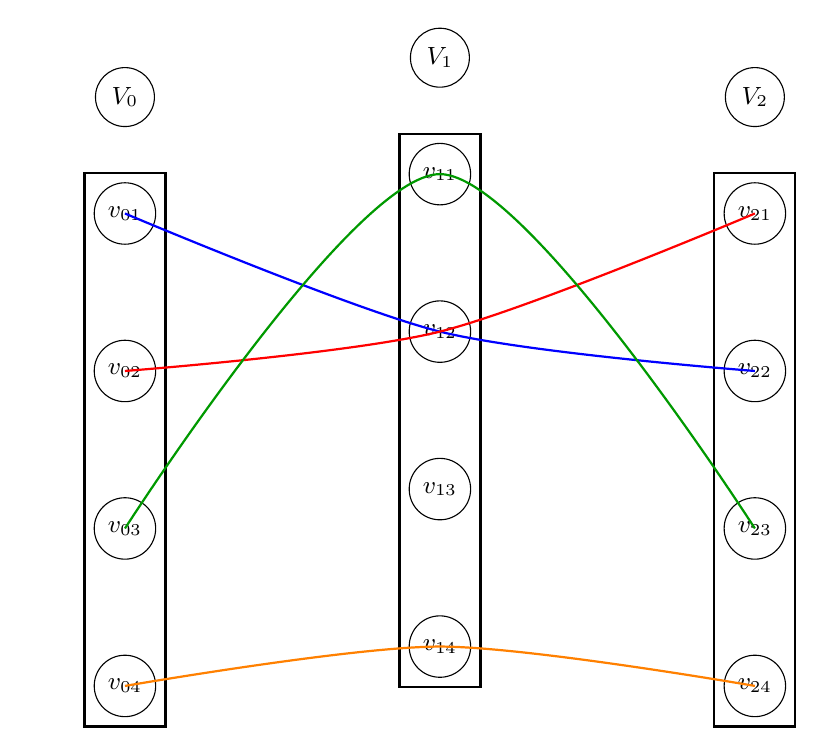
\begin{tikzpicture}[
  every node/.style={circle, draw, minimum size=7mm, font=\small},
  edge/.style={thick, bend left=15}
]

\node (v01) at (0,3) {$v_{01}$};
\node (v02) at (0,1) {$v_{02}$};
\node (v03) at (0,-1) {$v_{03}$};
\node (v04) at (0,-3) {$v_{04}$};

\node (v11) at (4,3.5) {$v_{11}$};
\node (v12) at (4,1.5) {$v_{12}$};
\node (v13) at (4,-0.5) {$v_{13}$};
\node (v14) at (4,-2.5) {$v_{14}$};

\node (v21) at (8,3) {$v_{21}$};
\node (v22) at (8,1) {$v_{22}$};
\node (v23) at (8,-1) {$v_{23}$};
\node (v24) at (8,-3) {$v_{24}$};

\node[above=0.7cm of v01] {$V_0$};
\node[above=0.7cm of v11] {$V_1$};
\node[above=0.7cm of v21] {$V_2$};

\begin{pgfonlayer}{background}
  \node[draw, thick, shape=rectangle, fit=(v01) (v02) (v03) (v04), label=left:{}] {};
  \node[draw, thick, shape=rectangle, fit=(v11) (v12) (v13) (v14), label=left:{}] {};
  \node[draw, thick, shape=rectangle, fit=(v21) (v22) (v23) (v24), label=left:{}] {};
\end{pgfonlayer}

\draw[thick, color=blue, smooth]
  plot coordinates {(v01) (v12) (v22)};

\draw[thick, color=red, smooth]
  plot coordinates {(v02) (v12) (v21)};

\draw[thick, color=green!60!black, smooth]
  plot coordinates {(v03) (v11) (v23)};

\draw[thick, color=orange, smooth]
  plot coordinates {(v04) (v14) (v24)};

\end{tikzpicture}

\caption{\centering Example of hypergraph with sets of vertices $V_0 = [v_{01}, v_{02}, v_{03}, v_{04}], V_1 = [v_{11}, v_{12}, v_{13}, v_{14}], V_2 = [v_{21}, v_{22}, v_{23}, v_{24}]$ and hyperedges $E = \{(v_{01}, v_{12}, v_{22}), (v_{02}, v_{12}, v_{21}), (v_{03}, v_{11}, v_{23}), (v_{04}, v_{14}, v_{24})\}$}
\end{figure}

Give a polynomial-time reduction of 3dCompleteMatching to SAT that, on hypergraphs with $n=|V_0|+|V_1|+|V_2|$ vertices and $m=|E|$ hyperedges, makes one oracle query on a formula with $m$ variables and $O(n + m^2)$ clauses. Clearly describe your preprocessing (what the variables represent and what clauses you construct), the oracle call, and your postprocessing (including what you return if the oracle returns $\bot$).

\textbf{You do not need to prove the correctness of your reduction or analyze its runtime.} \emph{Please keep your response within 12 sentences.}

Thus, even though the fastest known algorithms for 3dCompleteMatching run in exponential time, we can use SAT Solvers to solve it much more efficiently on many instances that arise in practice.

\begin{soln}
Let's define our variables: $x_i=1$ means hyperedge $i$ is in our solution $M$. As many variables as hyperedges means we have $m$ variables.

Our clauses are:
\begin{align}
	(\neg x_i \lor \neg x_j) && \text{for all $i\neq j$ that share a vertex} \\
	(\bigvee x_i) && \text{for all $v\in V_0$, for all hyperedges $i$ containing $v$}
\end{align}

The first set of clauses are constructed by checking all pairs of hyperedges in $E$ for a shared vertex for $O(m^2)$ clauses. The second set are constructed by iterating through all hyperedges in $E$ and adding each one to the clause for its $V_0$ member for $O(n)$ clauses. So we have a total of $O(n+m^2)$ clauses over $m$ variables.

At this point, if any of our clauses are empty, we can return $\bot$ -- i.e. a $V_0$ vertex has no possible matches.

Calling our oracle on the conjunction of all our clauses, a $\bot$ return means there is no complete 3-D matching and we likewise return $\bot$. Otherwise, we are returned a satisfying solution to our clauses, and for each flagged variable, we add the corresponding hyperedge to our solution set and return the final result.
\end{soln}

 \item (EthiCS reflection) Suppose you are given a bipartite graph $G=(V,E)$ representing possible kidney donor--recipient matches, where the edges represent perfect compatibility matches, with far fewer donors than recipients, and for which there are multiple \MaximumMatching\ solutions. No living donors in the graph face any health risks from the procedure. Finally, you have access to the following data for all of the potential recipients: (1) expected life years gained from transplant, (2) expected QALYs gained from transplant, (3) age, (4) past QALYs lived to date, and (5) household income. You are tasked with developing a metric $\val$ that takes some (or all) of that data
 and a potential matching $M\subseteq E$ and outputs a score $\val(M)\in \R$.
 Then your engineers will design an algorithm that finds a matching maximizing $\val(M)$.

 Describe some core characteristics your metric $\val$ ought to have and explain why you think those characteristics are ethically justified, drawing from at least one concept or discourse from the ethical \& social considerations lecture/chapter as well as your personal judgment.

 \textit{Note: As with the previous psets, you may include your answer in your PDF submission, but the answer should ultimately go into a separate Gradescope submission form.}
 
 \emph{Good responses are usually around 10 sentences}

\begin{soln}
With so many factors at play (i.e. life is complicated), the ethical decisions involved become impossible to determine an objective measure. For example, household income could be interpreted as a positive, neutral, or negative for a recipient score: Harvard Econ teaches that life satisfaction correlates with wealth, so would matching richer recipients be a utilitarian choice? Or should equity factor into the decision because lower incomes causes worse health, and to be fair QALY should favor lower income people? Or is life sacred and immeasurable, so none of these factors should be accounted for at all? Worst of all is the weighting of these factors, where the ethics of "What is one past year worth compared to one future year" is foggy when choosing between 0.45 and 0.46 and people die and live by that number. Each provided factor is also super murky, so in this case I would choose a simple metric: maximize QALYs. Unless a specific factor has an obvious or overwhelming reason to weight it one way or the other, simplicity on a nearer-to-objective measure like QALY is what I would say is the best course of action. However, one of the most important questions should also be included in the data: "Given your likely outcome and risks of a transplant, how much do you want the transplant? How much do you want to live X more years in Y condition?"
\end{soln}

\item Once you're done with this problem set, please fill out \href{https://forms.gle/qQp9CyLP9T4hMacMA}{this survey} so that we can gather students' thoughts on the problem set, and the class in general. It's not required, but we really appreciate all responses!

\end{enumerate}

\end{document}
